%&pdflatex
\section{Impostazione della lingua}
La prima schermata che ci darà l'installer di Debian è mostrata in Figura \vref{fig:language-selection}.

\begin{figure}[ht]
	\centering
	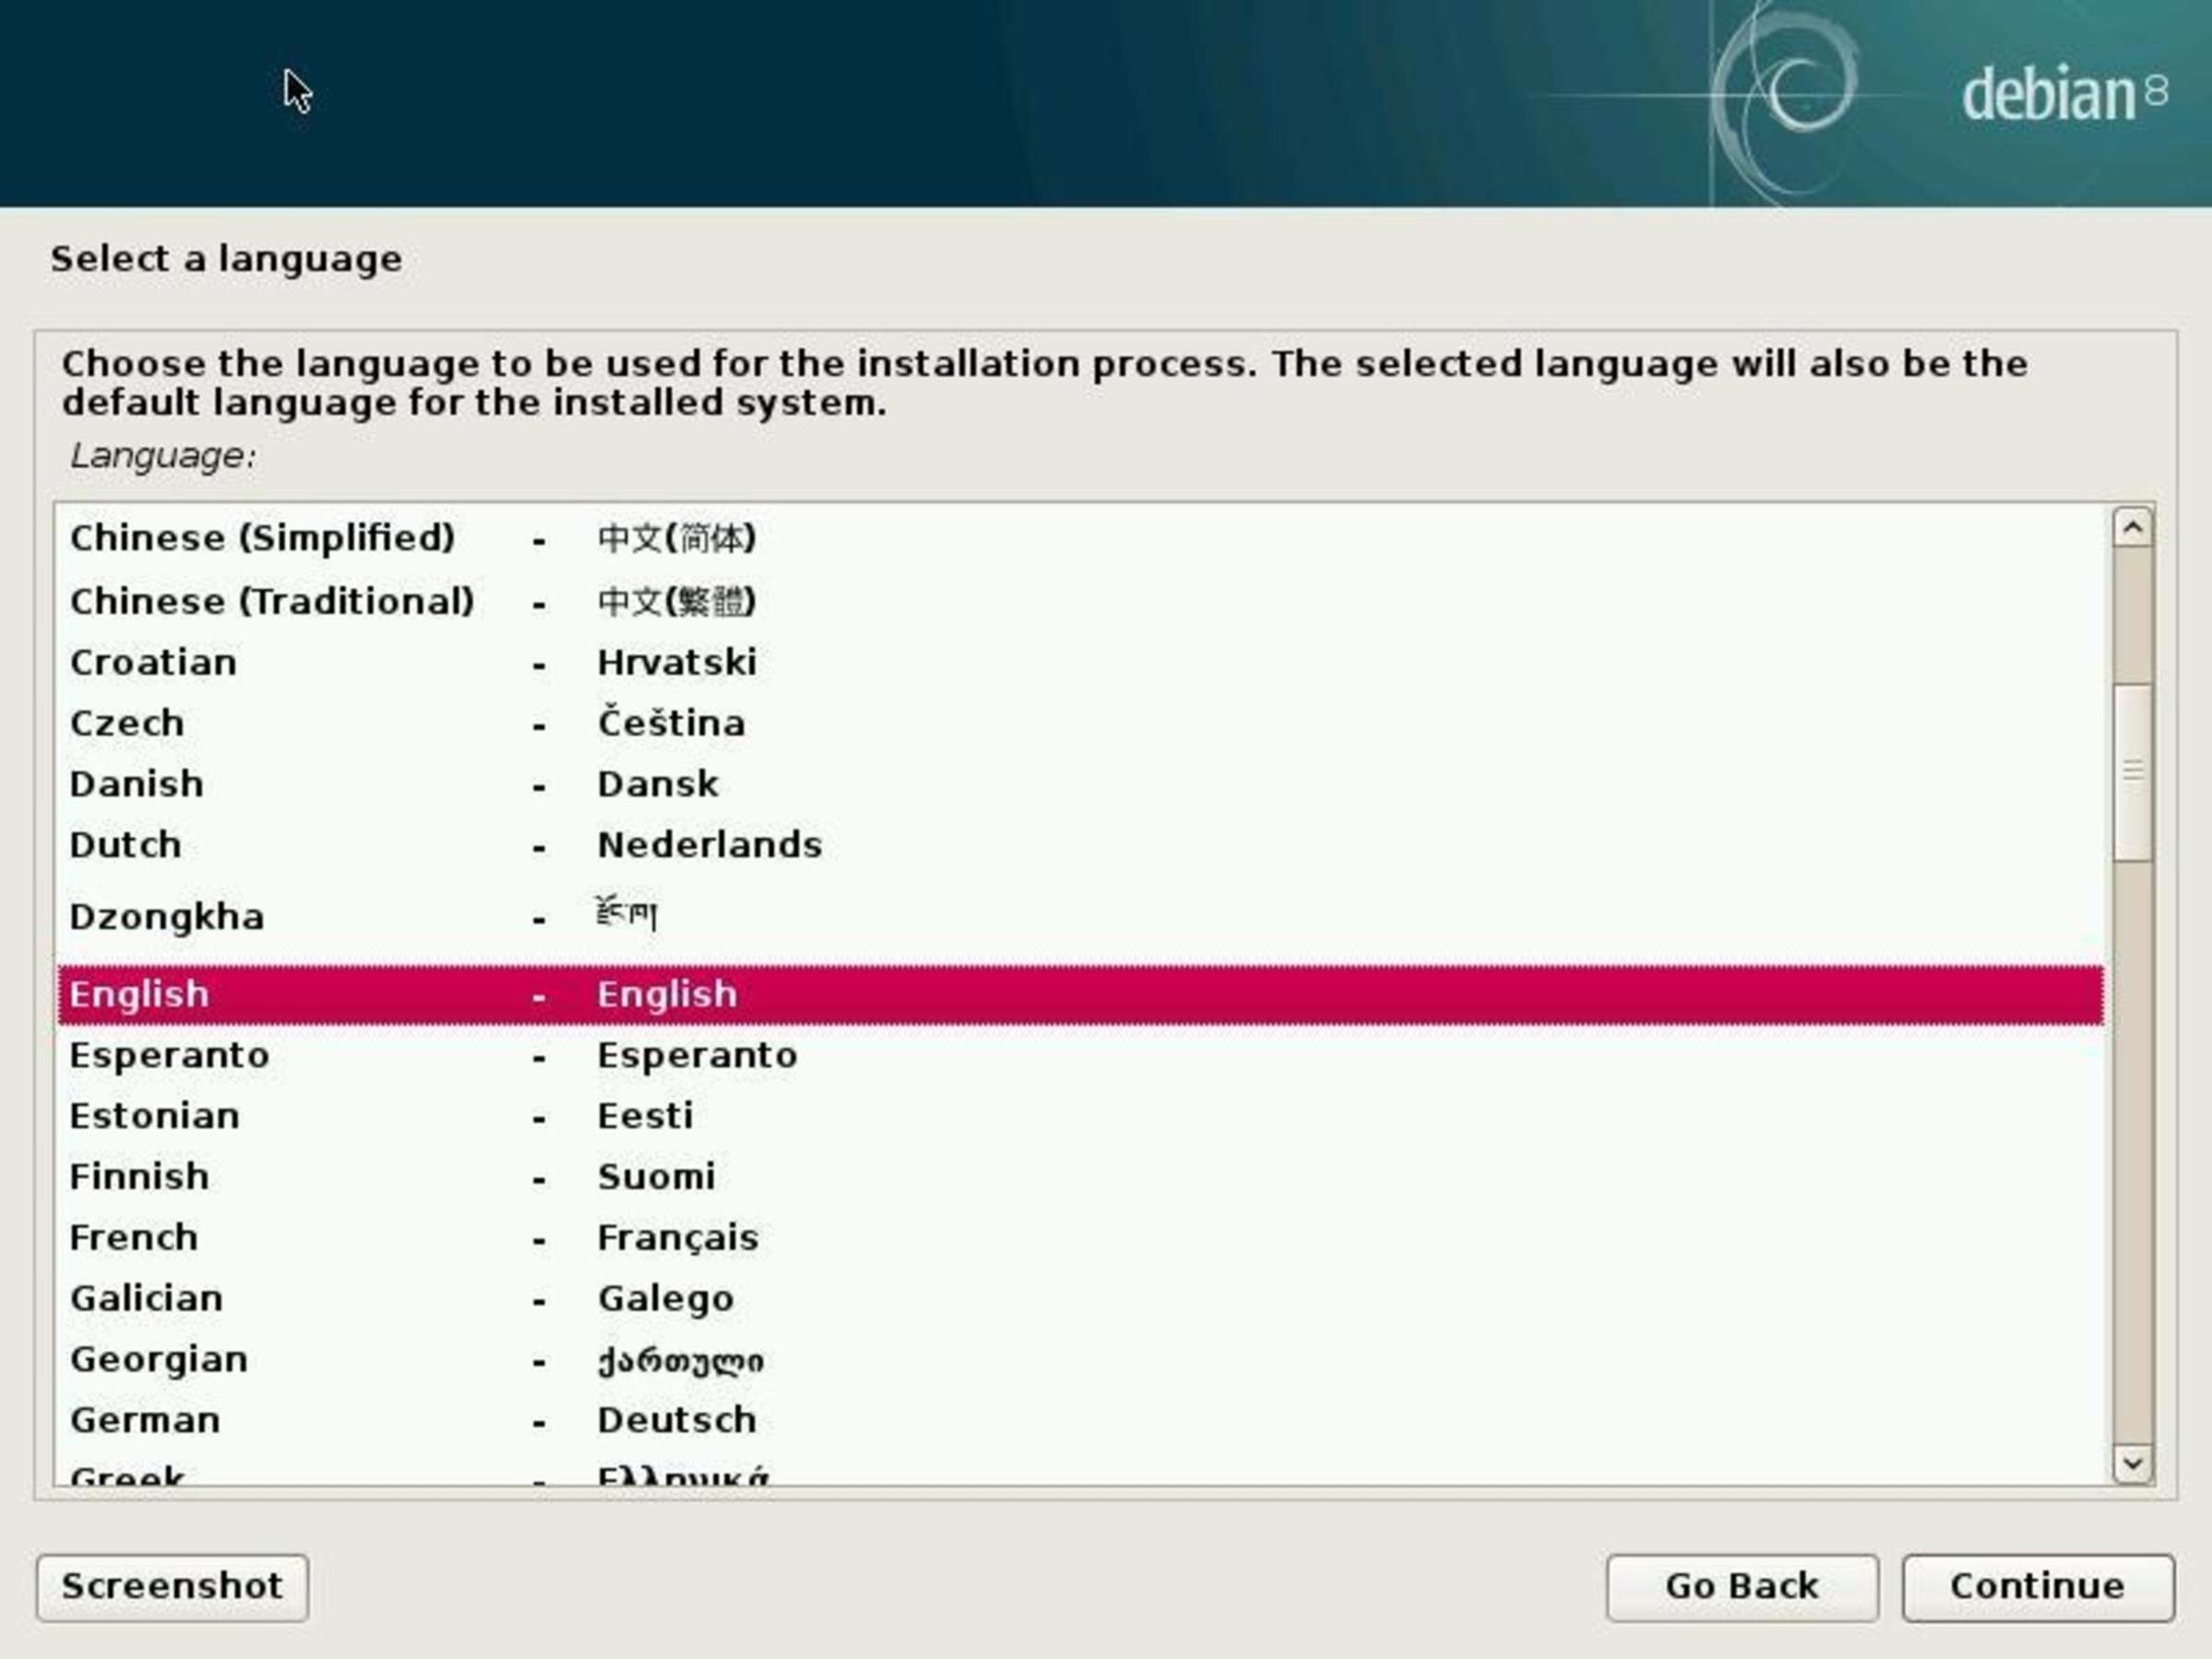
\includegraphics[resolution=600]{language-selection}
	\caption{Selezione della lingua}
	\label{fig:language-selection}
\end{figure}

Tra le lingue è disponibile anche l'italiano. Consigliamo però, se non si hanno problemi con la lingua inglese, di selezionare l'inglese: in tal modo in caso di problemi con il software, i \textit{log} dei programmi saranno mostrati in lingua inglese, permettendo quindi di chiedere assistenza nelle community internazionali di Linux mostrando i log in inglese. Ad ogni modo, il lettore può scegliere \texttt{Italiano} se preferisce. Una volta scelta la lingua, cliccare su \texttt{Continue}.

Nella schermata successiva viene chiesto di scegliere la propria zona per impostare correttamente l'ora secondo il fuso orario locale. Se al passaggio precedente si è scelto la lingua italiana, dovrebbe essere adesso comparsa la voce \texttt{Italia}. Se invece si è scelto, come consigliato, la lingua inglese, allora è necessario selezionare in ordine: \texttt{other} (in fondo alla lista) > \texttt{Europe} > \texttt{Italy}.

Successivamente, se si è scelto come lingua l'inglese e come zona l'Italia, l'installer ci chiederà quale locale utilizzare. Scegliamo \texttt{United States - en\_US.UTF-8} come mostrato in Figura \vref{fig:locale-selection}.

\begin{figure}[ht]
	\centering
	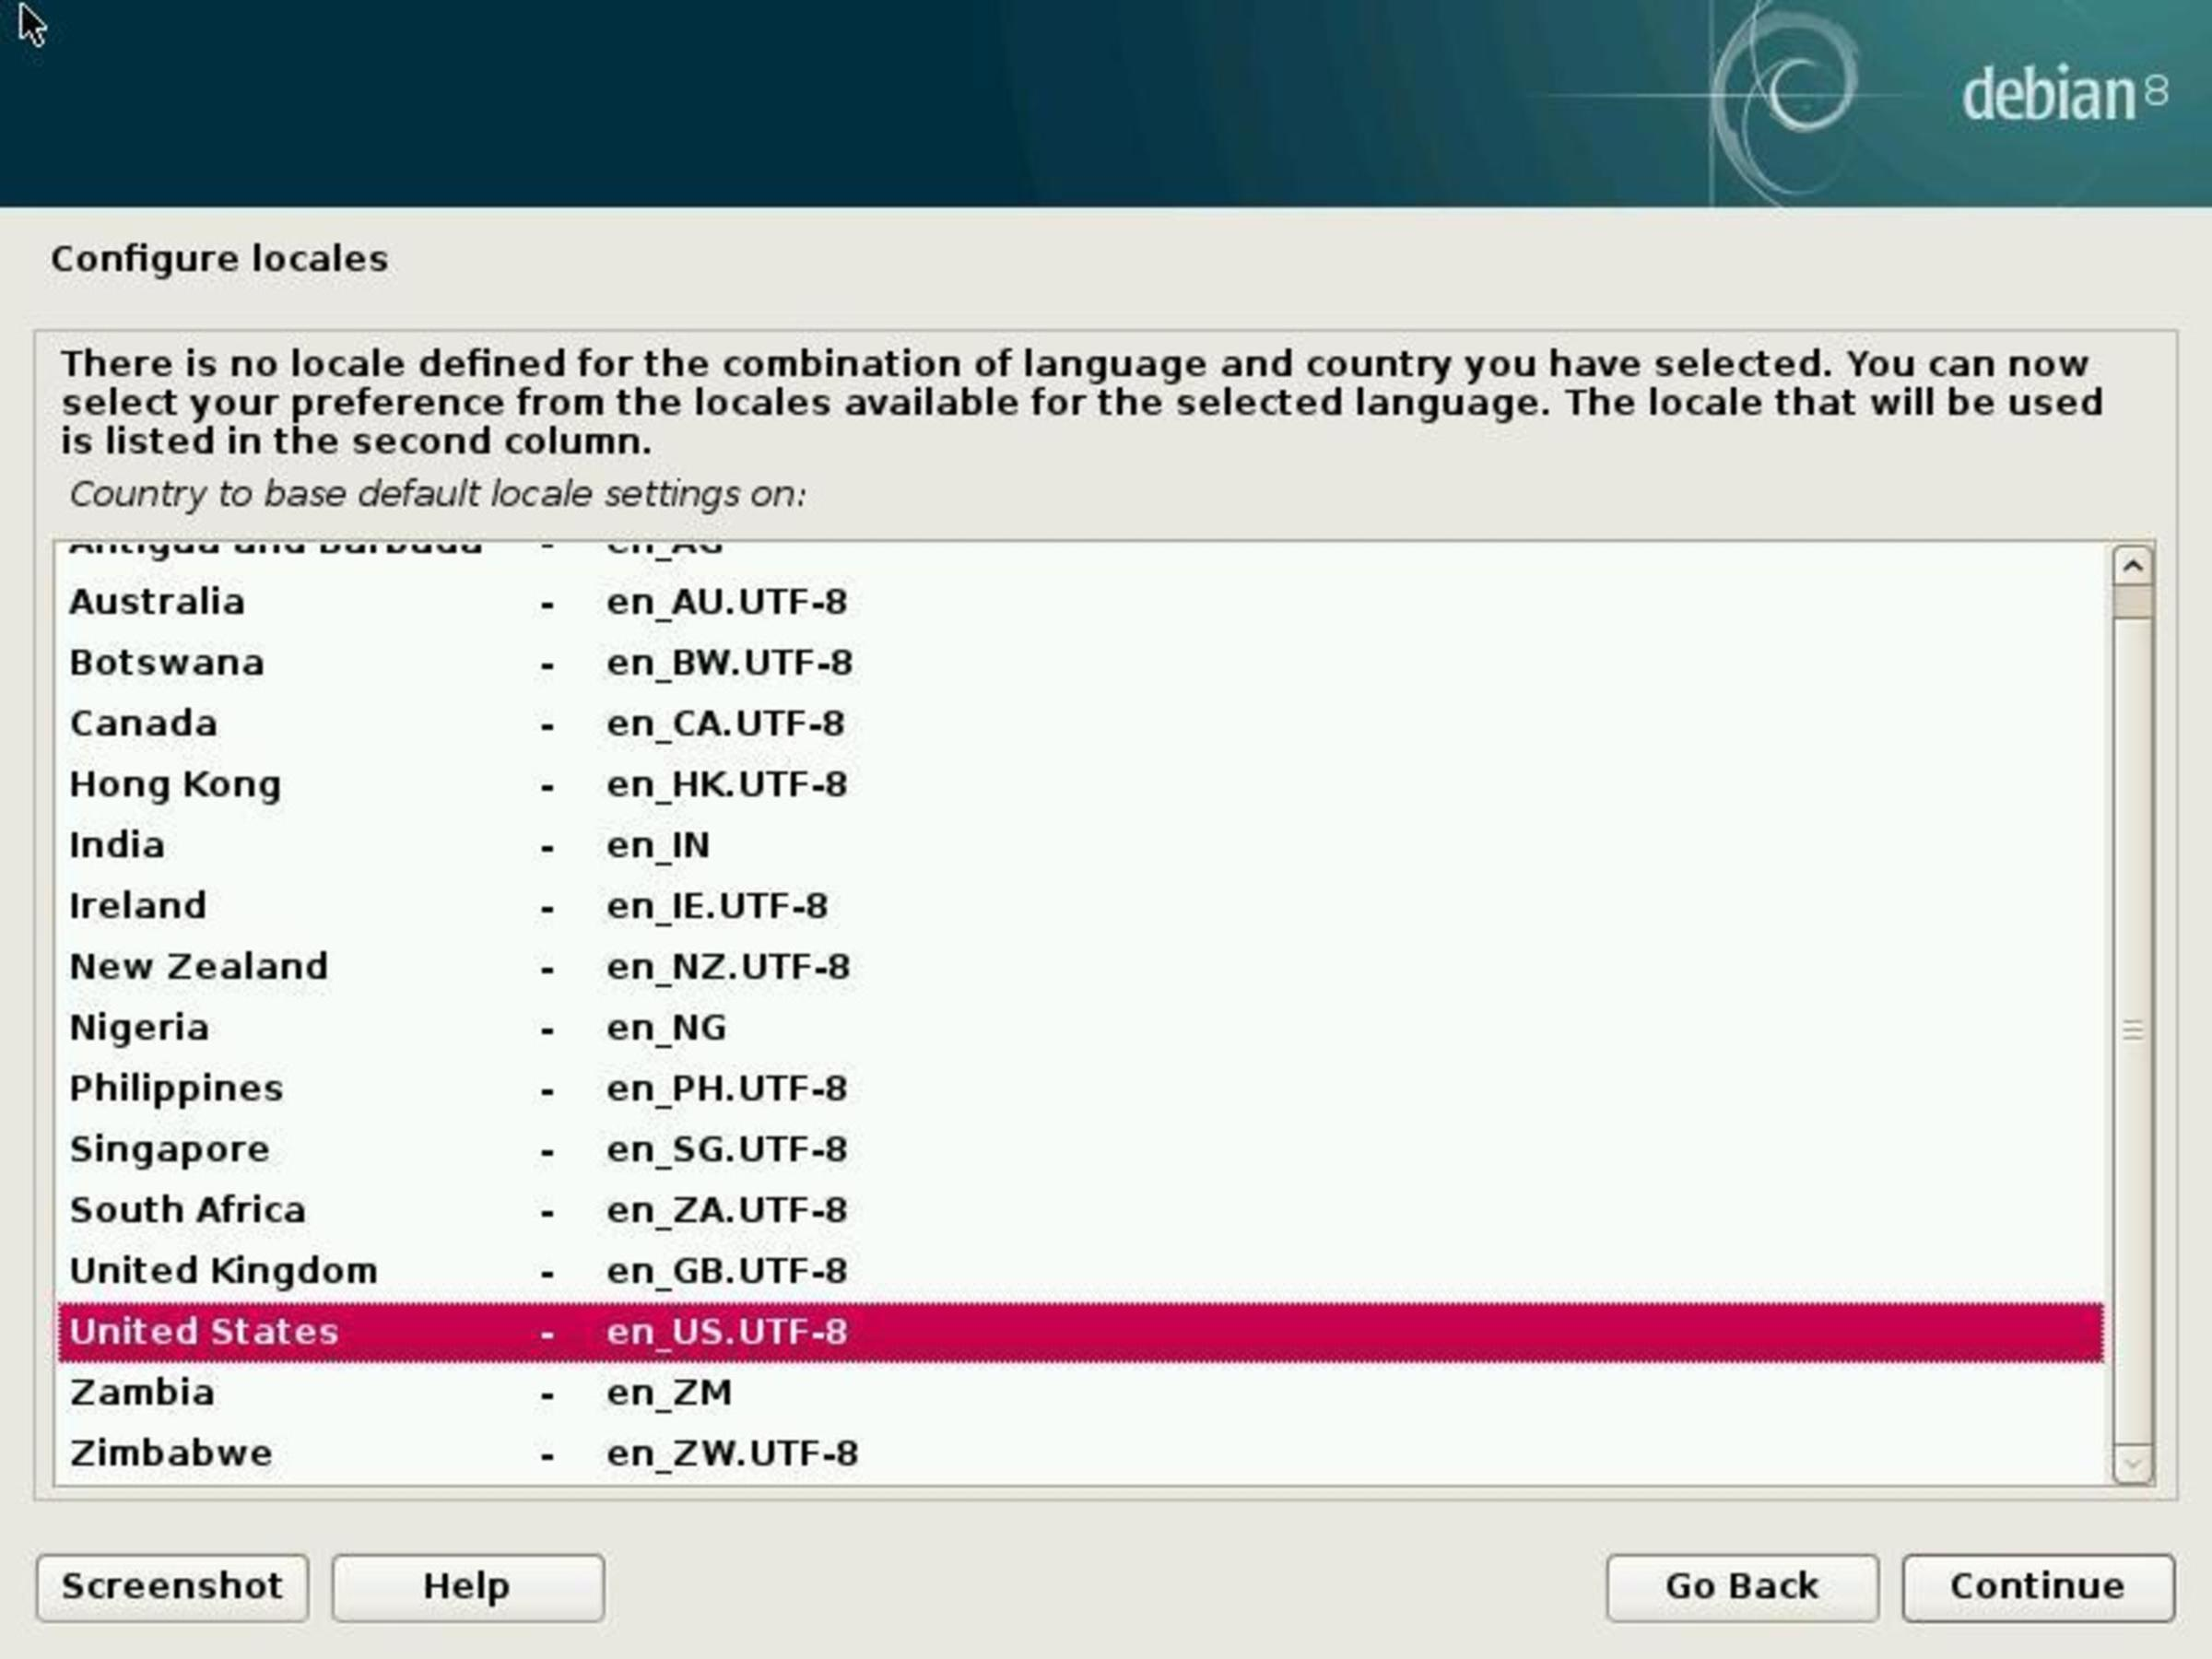
\includegraphics[resolution=600]{locale-selection}
	\caption{Selezione del locale}
	\label{fig:locale-selection}
\end{figure}

Se invece si è scelto come lingua l'italiano e come zona l'Italia, verrà selezionato automaticamente \texttt{Italia - it\_IT.UTF-8}.

Infine, ci verrà chiesto di selezionare il \textit{layout di tastiera}. Scegliamo \texttt{Italian} (\texttt{Italiana}).
